\begin{frame}[noframenumbering]
    \frametitle{Implementation}

    \begin{itemize}
        \item OpenAI Gym environment interface.
        \item Custom proximal policy optimization implementation.
        \item PyTorch for models and automatic differentiation.
        \item Intel Core i9-10900X CPU.
        \item NVIDIA GeForce RTX 2080 Ti GPU.
    \end{itemize}
\end{frame}

\begin{frame}[noframenumbering]
    \frametitle{Search Paths I}

    \begin{columns}
        \begin{column}{0.5\textwidth}
            \begin{figure}
                \centering
                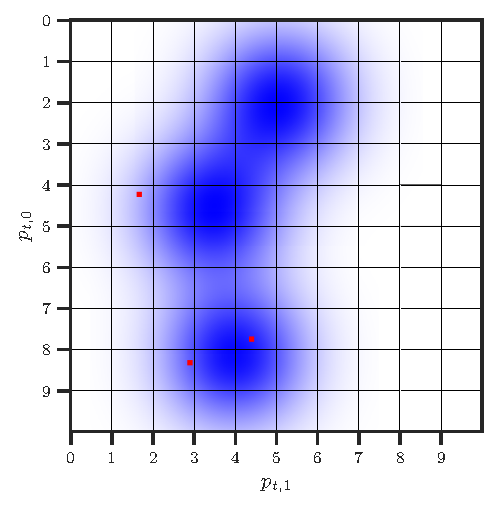
\includegraphics[scale=0.5]{figures/path-scene.pdf}
                \par Environment sample
            \end{figure}
        \end{column}
        \begin{column}{0.5\textwidth}
            \begin{figure}
                \centering
                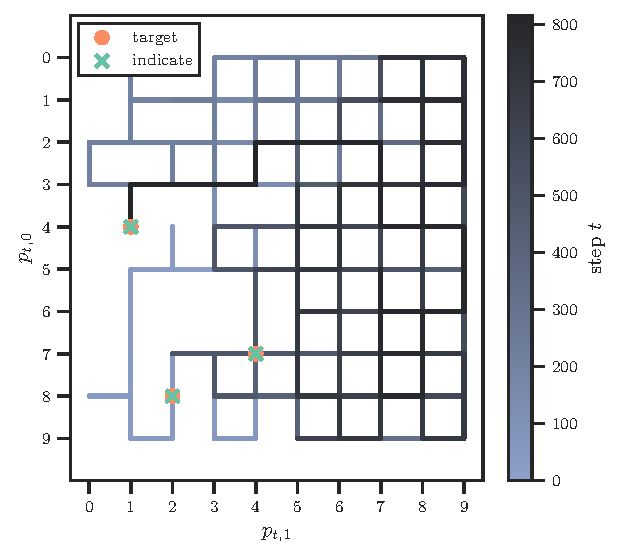
\includegraphics[scale=0.5]{figures/path-random.pdf}
                \par Random baseline
            \end{figure}
        \end{column}
    \end{columns}
\end{frame}

\begin{frame}[noframenumbering]
    \frametitle{Search Paths II}

    \begin{columns}
        \begin{column}{0.5\textwidth}
            \begin{figure}
                \centering
                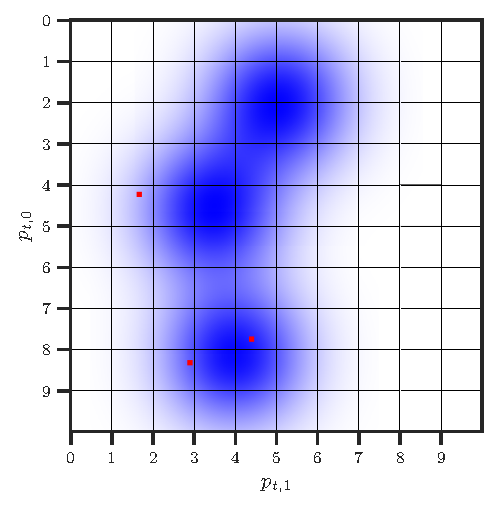
\includegraphics[scale=0.5]{figures/path-scene.pdf}
                \par Environment sample
            \end{figure}
        \end{column}
        \begin{column}{0.5\textwidth}
            \begin{figure}
                \centering
                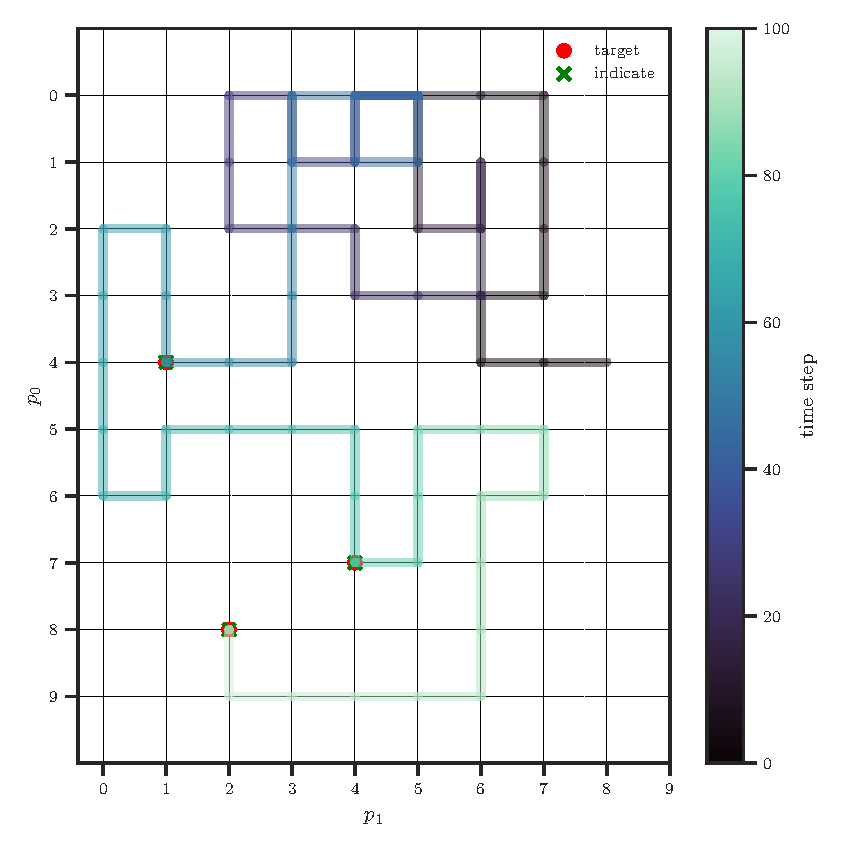
\includegraphics[scale=0.5]{figures/path-greedy.pdf}
                \par Greedy baseline
            \end{figure}
        \end{column}
    \end{columns}
\end{frame}

\begin{frame}[noframenumbering]
    \frametitle{Search Paths III}

    \begin{columns}
        \begin{column}{0.5\textwidth}
            \begin{figure}
                \centering
                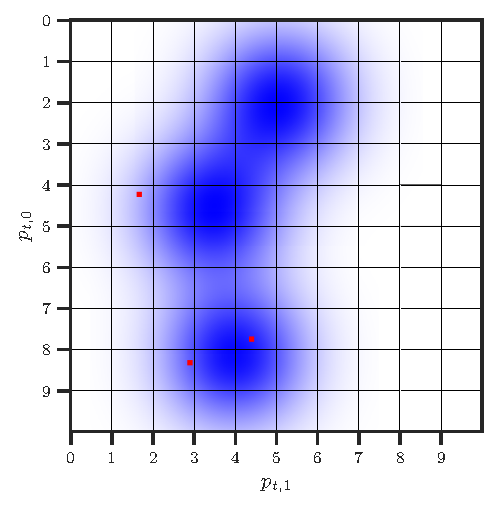
\includegraphics[scale=0.5]{figures/path-scene.pdf}
                \par Environment sample
            \end{figure}
        \end{column}
        \begin{column}{0.5\textwidth}
            \begin{figure}
                \centering
                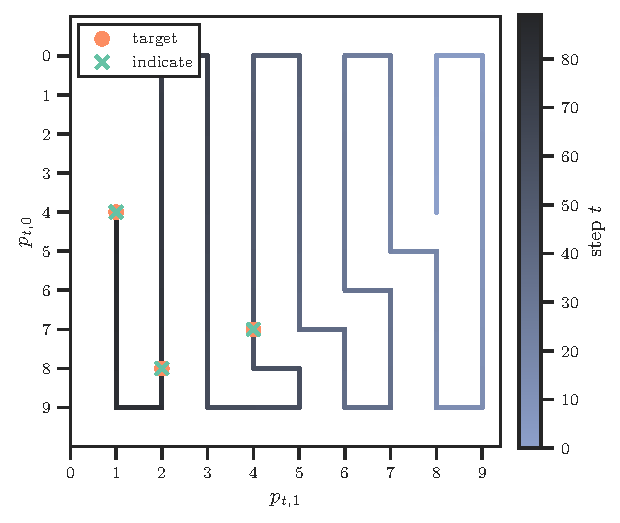
\includegraphics[scale=0.5]{figures/path-exhaustive.pdf}
                \par Exhaustive baseline
            \end{figure}
        \end{column}
    \end{columns}
\end{frame}

\begin{frame}[noframenumbering]
    \frametitle{Search Paths IV}

    \begin{columns}
        \begin{column}{0.5\textwidth}
            \begin{figure}
                \centering
                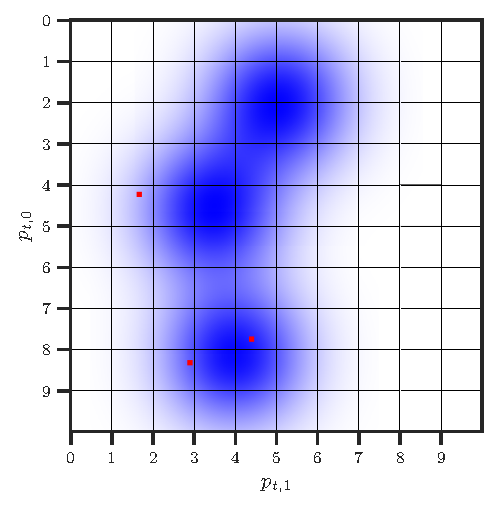
\includegraphics[scale=0.5]{figures/path-scene.pdf}
                \par Environment sample
            \end{figure}
        \end{column}
        \begin{column}{0.5\textwidth}
            \begin{figure}
                \centering
                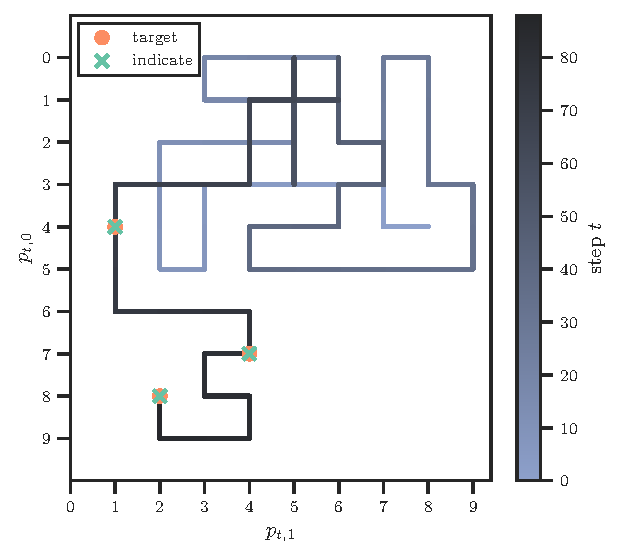
\includegraphics[scale=0.5]{figures/path-handcrafted.pdf}
                \par Handcrafted baseline
            \end{figure}
        \end{column}
    \end{columns}
\end{frame}

\begin{frame}[noframenumbering]
    \frametitle{Search Paths V}

    \begin{columns}
        \begin{column}{0.5\textwidth}
            \begin{figure}
                \centering
                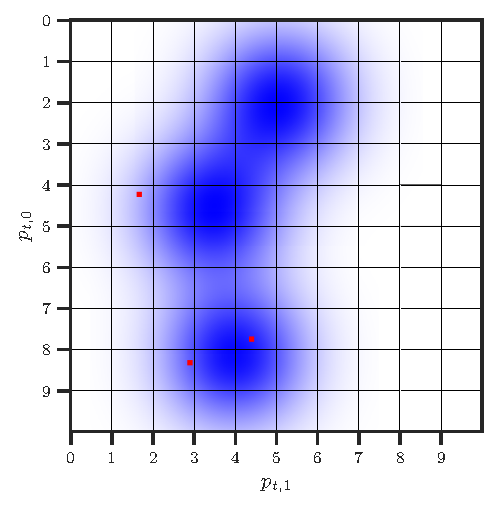
\includegraphics[scale=0.5]{figures/path-scene.pdf}
                \par Environment sample
            \end{figure}
        \end{column}
        \begin{column}{0.5\textwidth}
            \begin{figure}
                \centering
                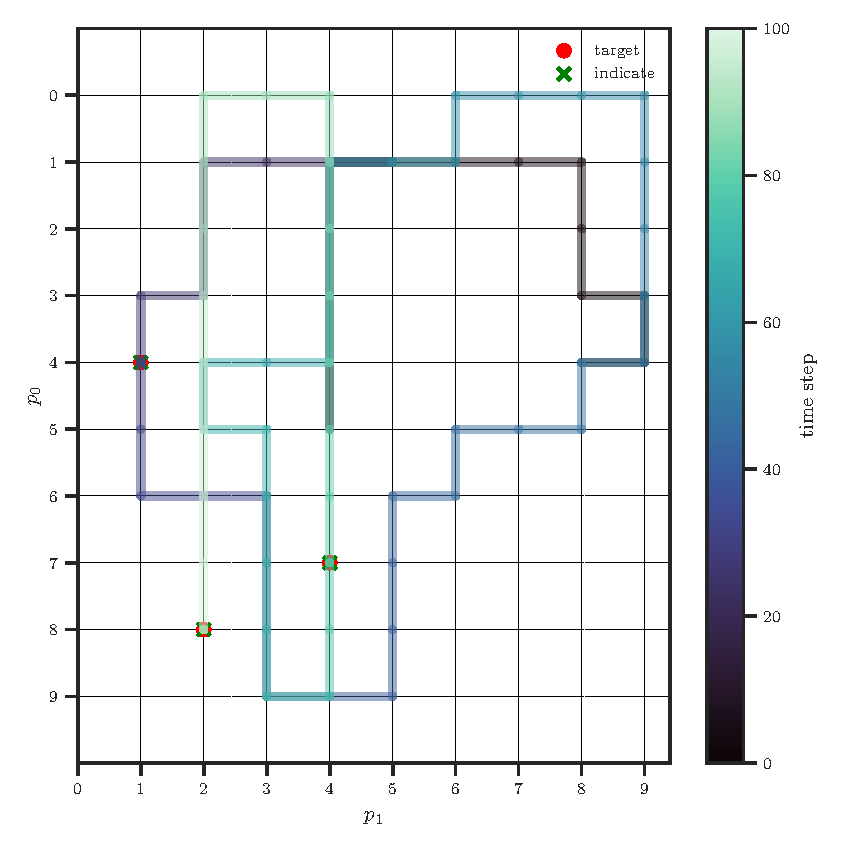
\includegraphics[scale=0.5]{figures/path-lstm.pdf}
                \par Temporal memory
            \end{figure}
        \end{column}
    \end{columns}
\end{frame}

\begin{frame}[noframenumbering]
    \frametitle{Search Paths VI}

    \begin{columns}
        \begin{column}{0.5\textwidth}
            \begin{figure}
                \centering
                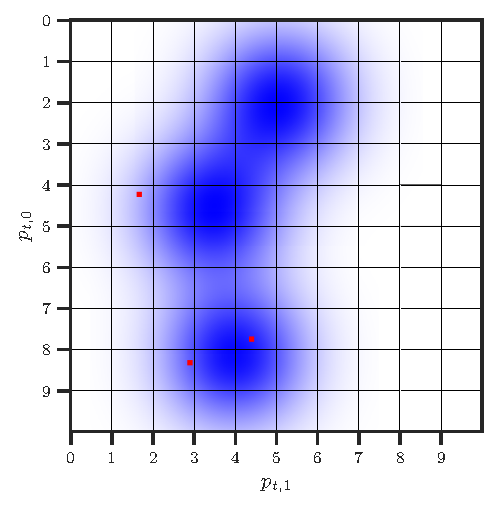
\includegraphics[scale=0.5]{figures/path-scene.pdf}
                \par Environment sample
            \end{figure}
        \end{column}
        \begin{column}{0.5\textwidth}
            \begin{figure}
                \centering
                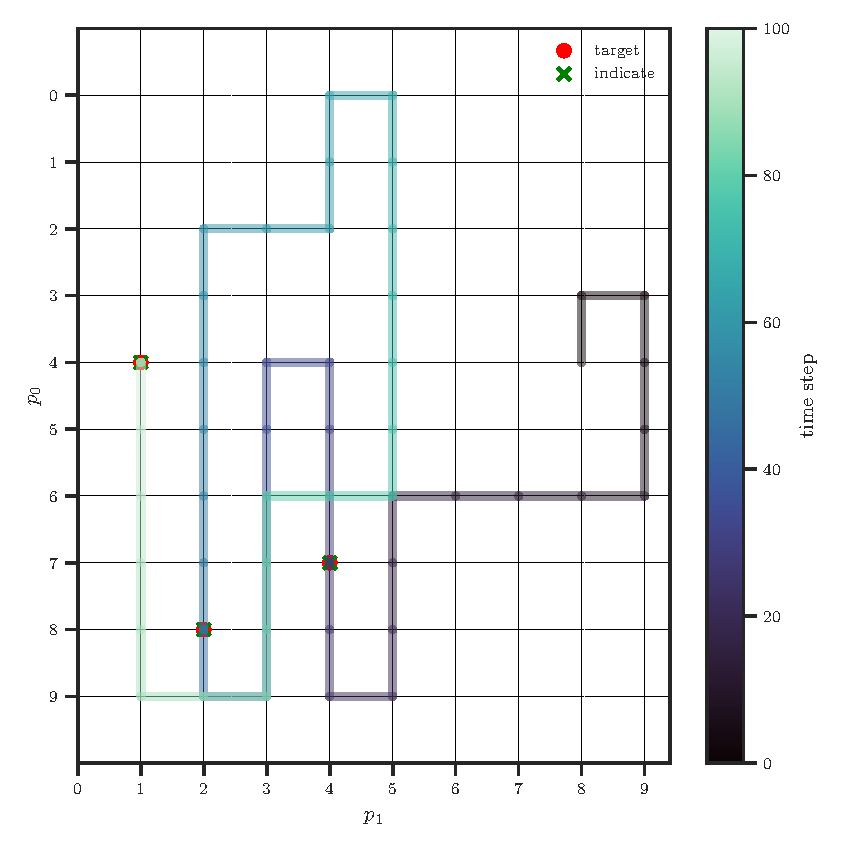
\includegraphics[scale=0.5]{figures/path-map.pdf}
                \par Spatial memory 
            \end{figure}
        \end{column}
    \end{columns}
\end{frame}

\begin{frame}[noframenumbering]
    \frametitle{Memory Viualization}

    \begin{figure}
        \centering
        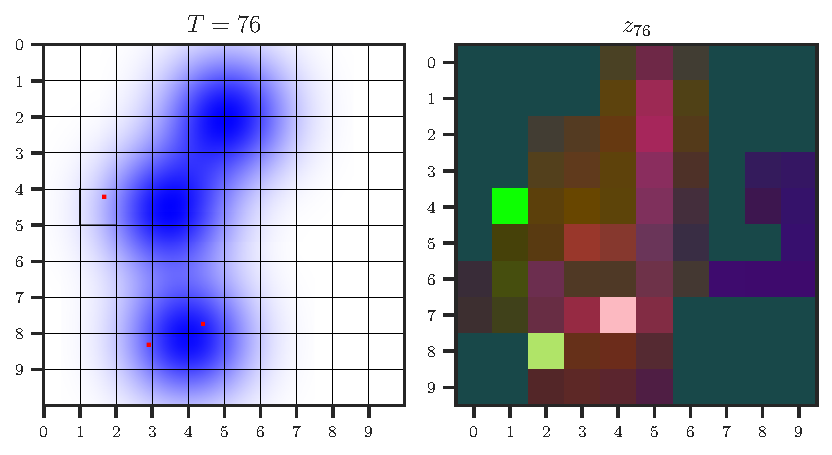
\includegraphics[scale=0.75]{figures/memory-map.pdf}
        \par PCA decomposition of spatial memory after episode.
    \end{figure}
\end{frame}
